\documentclass[11pt]{article}

\usepackage[margin=1in]{geometry}
\usepackage[T1]{fontenc}
\usepackage[utf8]{inputenc}
\usepackage{lmodern}
\usepackage{amsmath}
\usepackage{booktabs}
\usepackage{array}
\PassOptionsToPackage{hyphens}{url}
\usepackage{hyperref}
\renewcommand{\UrlBreaks}{\do\/\do\-\do\_\do\.}
\usepackage{longtable}
\usepackage{graphicx}
\usepackage{setspace}

\title{Target-Conditioned Corpus Transformation: A Non-Neural Typological Projection}
\author{Taylor Osborn \\ Independent Researcher}
\date{Draft: May 4, 2026}

\begin{document}

\maketitle

\begin{abstract}
This paper documents a frozen French $\rightarrow$ Latin production run in
Project RBT, a non-neural corpus transformation system that operates on
corpus-level statistical fingerprints rather than cognate lists, sound laws,
or explicit morphological supervision. The active system is target-conditioned:
modern French is the source corpus and Latin provides the in-loop structural
and form reference. Languages are represented through token co-occurrence,
positional distributions, word n-gram profiles, and character-level form
profiles. The reported \emph{v5} run used 16 candidates per proposal, block
size 1000, incremental scoring, and Fortran-accelerated hot-loop components.
It halted natively by a plateau rule after 614{,}000 proposals. The final
Latin structural score was $-0.00010808926278147055$ (bounded above by
zero, with zero indicating an exact match), the final Latin form score
was $0.7611594796180725$, and the final family alignment score was
$0.513866759690557$ (approximately $54\%$ of the achievable Latin ceiling
under the active scoring function; see Limitations). The best form
checkpoint occurred earlier in the run at
block 338 with a Latin form score of $0.8632466197013855$. Post hoc comparison
against a held-out validator bank of six attested medieval Romance corpora
showed a structural nearest-neighbor path that oscillated between Middle
French and Old Spanish during the first half of the run before settling on
Old Occitan in the second half, and a form nearest-neighbor path that
alternated between Middle French and other langue d'o\"il varieties. The paper
reports the computational setup, stopping rule, preserved checkpoints, and
validator-bank outputs for this run. A post hoc dimensional robustness
check additionally places Sumerian, a non-Indo-European language
unrelated to Romance, at fourth-rank structural proximity to Latin; we
read the structural metric as a typological proximity detector rather
than a chronological one.
\end{abstract}

\section{Introduction}

Project RBT studies target-conditioned statistical retrodiction in historical
linguistic space. In the present configuration, a modern descendant corpus is
iteratively mutated under explicit pressure from a historical target corpus,
and the resulting synthetic states are compared against held-out attested
historical corpora after the run completes. Most quantitative approaches to historical linguistic reconstruction
operate on discrete lexical units: Bayesian phylogenetic methods using
cognate sets and sound correspondences~\cite{bouchardcote2013,bouckaert2012},
cognate-detection algorithms and standardized lexical databases for
comparative work~\cite{forkel2018}, statistical models of language change
at the lexeme level~\cite{pagel2007}, and computational-phylogenetic
surveys that chart the methodological landscape~\cite{bowern2018}. The
system reported here is different in kind: it operates on corpus-level
statistical fingerprints (n-gram coverage, type-token statistics,
character profiles, and suffix profiles) and makes no use of cognate
alignments, sound laws, or hand-curated correspondences. The empirical
interest of the trajectory lies in what intermediate states the
fingerprint geometry produces under target pressure, not in what
historical processes those states represent.

Many quantitative approaches to historical linguistic comparison and
reconstruction now incorporate neural components, from Bayesian phylogenetic
methods with neural posteriors to transformer-based cognate detection. The
approach reported here is deliberately non-neural for three reasons. First,
every feature in the structural and form scoring paths has an explicit
statistical interpretation that can be read directly from a corpus and
traced back from any score; this transparency is harder to achieve with
learned embeddings. Second, the engine runs on CPU, is fully deterministic
given a seed, and has no GPU, framework-version, or pre-trained-model
dependencies; the v5 run reported below completed in approximately 135
hours of CPU compute and can be reproduced on commodity hardware. Third,
the research question being investigated, what intermediate states a
corpus-level fingerprint geometry produces under target pressure, is a
property of the metric space rather than a predictive task; neural methods
are well-suited to optimizing predictive accuracy on held-out test sets,
but the question explored here is different in kind.

The present paper is descriptive in scope. It documents one frozen production
run from modern French toward Latin and reports three classes of output:

\begin{enumerate}
    \item the computational and statistical method used for the run,
    \item the endpoint and checkpoint metrics produced by the run, and
    \item the post hoc validator-bank comparison against attested historical
    corpora not used in the optimization loop.
\end{enumerate}

The paper does not claim blind reconstruction. Latin is in the optimization
loop as the active target reference, and the run is therefore reported as a
target-conditioned retrodictive search rather than as unsupervised ancestor
recovery.

The present paper is best read as an instrument study rather than a
contribution to historical-linguistic reconstruction. Language was chosen
as the test domain because attested historical Romance corpora are available
as held-out validators and because the author has a research interest in
computational historical linguistics; the engine and the structural scoring path are
likely agnostic to domain in their underlying structure and could in principle be
applied to other corpus-statistical comparison tasks; the family alignment
component, however, is specific to linguistic data. The contribution made
here is therefore methodological: it documents a target-conditioned search
over a specific four-dimensional feature space, the empirical behavior of
that search against a held-out validator bank, and the metric-space
properties that emerge under expansion to a richer feature space. The
historical-linguistic content of those findings is a consequence of the
chosen input data and active reference set, not a claim about Romance
language change. The paper does not model historical language change in
the wild: the transmission, contact, and innovation processes by which
languages actually transform over time. The engine operates on corpus-level
statistical features and is silent on those processes.

\section{Materials and Methods}

\subsection{Corpus roles}

The run reported here uses four corpus roles: source, target, held-out
validators, and controls. Table~\ref{tab:corpusroles} summarizes the role
assignment used in the project-level methodology.

\begin{table}[h]
\centering
\caption{Corpus roles used in the active methodology.}
\label{tab:corpusroles}
\begin{tabular}{p{1.8in}p{3.8in}}
\toprule
Role & Corpus set \\
\midrule
Source corpus & Modern French \\
In-loop target & Classical Latin \\
Held-out historical validators & Old French, Middle French, Anglo-Norman,
other langue d'o\"il varieties, Old Spanish / early Iberian, Old Occitan \\
Null and control corpora & Markov noise, Sumerian, withheld Portuguese \\
\bottomrule
\end{tabular}
\end{table}

The source corpus for the paper run was the processed modern French corpus in
\path{data/processed/romance/french_tokens.json}. Latin served as the active
reference for structural and form scoring. The validator bank was not used in
the search objective and was only applied after the run completed. Sumerian
was included in the control bank as a structured non-Indo-European control,
intended to distinguish engine-driven structural tracking from the
Markov-noise floor.

\subsection{Statistical representation}

Languages are represented as statistical fingerprints over tokenized corpora.
The active representation combines the following components:

\begin{enumerate}
    \item token co-occurrence structure,
    \item positional token distributions,
    \item word bigram and trigram profiles,
    \item type-token statistics,
    \item character bigram and trigram profiles, and
    \item suffix profiles.
\end{enumerate}

The structural side of the scoring path uses corpus-level structural vectors
derived from these token-distribution features. The form side uses
character-level profiles and suffix profiles. Candidate scoring in the engine
therefore tracks at least three quantities throughout the run:

\begin{itemize}
    \item Latin structural score,
    \item Latin form score,
    \item family alignment / coherence diagnostics.
\end{itemize}

\paragraph{Structural score.}
Each corpus state is projected onto a four-dimensional feature vector:
type--token ratio, top-100 bigram coverage, top-100 trigram coverage, and
$\log(1 + \overline{L})$ where $\overline{L}$ is the mean sequence length.
The structural score used as the in-loop search reward is the negative
Euclidean distance between the candidate's and the target's vectors
restricted to the first three features, scaled by $5.0$:
%
\begin{equation}
\label{eq:struct-score}
S_{\mathrm{struct}}
  = -5.0 \cdot \left\| \mathbf{v}_{\mathrm{cand}}^{[1:3]}
                - \mathbf{v}_{\mathrm{Latin}}^{[1:3]} \right\|_2.
\end{equation}
%
The fourth feature, $\log(1 + \overline{L})$, is excluded from the reward
because the candidate-generation path preserves the source sentence-length
distribution and cannot optimize that dimension directly. Zero indicates
an exact three-feature match; the score is bounded above by zero. The
full four-dimensional structural vector is retained for the post hoc
validator-bank comparison described in Section~2.6, which uses a
different distance function on a different reference set.

\paragraph{Form score.}
The form score combines three character-level cosine similarities against the
target:
\[
  S_{\mathrm{form}} =
    0.40 \cdot \cos(\mathbf{bg}_{\mathrm{cand}},\mathbf{bg}_{\mathrm{target}})
  + 0.40 \cdot \cos(\mathbf{tg}_{\mathrm{cand}},\mathbf{tg}_{\mathrm{target}})
  + 0.20 \cdot \cos(\mathbf{sf}_{\mathrm{cand}},\mathbf{sf}_{\mathrm{target}})
\]
where $\mathbf{bg}$ is the top-1{,}500 character bigram profile,
$\mathbf{tg}$ is the top-2{,}500 character trigram profile, and
$\mathbf{sf}$ is the top-800 three-character suffix profile.

\paragraph{Family alignment score.}
The family alignment score applies the Hungarian assignment
algorithm~\cite{kuhn1955} to match suffix and prefix families between the
candidate and the target, normalised to $[0, 1]$.

\subsection{Search configuration}

The run was executed through the \emph{v5} long-run driver. The active engine
inherits the \emph{v4} mutation-and-acceptance controller and adds the
\emph{v5} configuration surface. For the paper run, the search used the
configuration shown in Table~\ref{tab:runconfig}.

\begin{table}[h]
\centering
\caption{Frozen configuration for the French $\rightarrow$ Latin paper run.}
\label{tab:runconfig}
\begin{tabular}{ll}
\toprule
Parameter & Value \\
\midrule
Source language & French \\
Target language & Latin \\
Candidate count & 16 \\
Block proposals & 1000 \\
Number of sequences & 800 \\
Minimum improvement & 0.0001 \\
Structural target & 0.0 \\
Form target & 1.0 \\
Family target & 1.0 \\
Incremental scoring & on \\
Fortran cosine & on \\
Fortran batch & on \\
Semantic transparency & off \\
Transparency weight & 0.0 \\
Culture bombs & off \\
Validator snapshots during run & off \\
Live event mode & all \\
Requested launch seed & 45 \\
Audited engine seed & 42 \\
\bottomrule
\end{tabular}
\end{table}

Candidate proposals were evaluated under the active \emph{v5} weighted
objective. The total score for a candidate state combines the Latin
structural and form scores defined in \S2.2, a coherence margin against
the Markov-noise floor, the candidate's mutation cost, and a reward bonus
that rewards strict improvement along the structural, form, suffix, and
character-trigram axes:

\begin{equation}
\label{eq:v5objective}
S_{\text{total}}
= S_{\text{struct}}
+ w_f\,S_{\text{form}}
+ w_c\,M_{\text{coh}}
- w_m\,C_{\text{mut}}
+ R_{\text{bonus}}
+ R_{\text{relief}},
\end{equation}

with reward and relief terms

\begin{align*}
R_{\text{bonus}}  &= w_{\Delta s}\,[\Delta s]_+
                  + w_{\Delta f}\,[\Delta f]_+
                  + w_{\Delta\sigma}\,[\Delta\sigma]_+
                  + w_{\Delta\tau}\,[\Delta\tau]_+
                  + b_j\,\mathbf{1}_J, \\
R_{\text{relief}} &= w_r\,w_m\,C_{\text{mut}}\,\mathbf{1}_J,
\end{align*}

where $[x]_+ = \max(0, x)$; $\Delta s$, $\Delta f$, $\Delta\sigma$, and
$\Delta\tau$ are the changes in Latin structural score, Latin form score,
character suffix cosine, and character trigram cosine between the candidate
and the current accepted state; and $\mathbf{1}_J$ is the indicator for the
joint-gain condition $(\Delta s > 0) \wedge (\Delta f > 0) \wedge
(\Delta c \geq -\delta_c)$, with $\Delta c$ the coherence-margin gain and
$\delta_c$ a fixed tolerance configured separately. The numerical values
used for the paper run were:

\begin{itemize}
    \item $w_f = 0.75$ (form weight),
    \item $w_c = 0.05$ (coherence weight),
    \item $w_m = 0.005$ (mutation cost weight),
    \item $w_{\Delta s} = 8.0$ (reward struct gain weight),
    \item $w_{\Delta f} = 4.0$ (reward form gain weight),
    \item $w_{\Delta\sigma} = 2.0$ (reward suffix gain weight),
    \item $w_{\Delta\tau} = 2.0$ (reward trigram gain weight),
    \item $b_j = 0.01$ (reward joint bonus),
    \item $w_r = 1.0$ (reward penalty relief).
\end{itemize}

Accepted-stage dense artifact generation remained in the standard Python path.
The accelerated path moved hot-loop scoring work into incremental and
Fortran-assisted components without changing the run's methodological objective.

\subsection{Computational execution path}

Within each proposal cycle, the engine generated a fixed batch of candidate
mutations, scored those candidates under the active objective, accepted at most
one candidate, and then advanced to the next proposal. The paper run used the
following division of labor:

\begin{itemize}
    \item Python owned mutation generation, acceptance decisions, block
    control, artifact writing, and manifest updates.
    \item Incremental scoring state maintained rolling counters so that
    unchanged portions of the corpus did not need to be rescored from scratch
    on every candidate.
    \item Fortran-backed paths were enabled for cosine-heavy structural
    computations and candidate-batch structural scoring.
    \item Dense accepted-stage artifact generation remained in the Python path
    and was only performed for committed stages rather than for every rejected
    candidate.
\end{itemize}

This split preserves a single methodological objective while moving the
highest-frequency numeric work into the accelerated path.

\subsection{Stopping rule}

The run used indefinite total budget (\texttt{total\_target\_proposals = 0})
with plateau-based stopping. The plateau rule operated over a window of 10
completed blocks. For each of the three monitored axes

\begin{itemize}
    \item Latin structural score,
    \item Latin form score,
    \item family alignment score,
\end{itemize}

the driver compared the best value observed in the most recent 10 blocks to the
best value observed in all prior blocks. Plateau was declared if none of the
three recent best values exceeded the earlier best by more than its threshold:

\begin{itemize}
    \item structural epsilon = 0.001,
    \item form epsilon = 0.001,
    \item family epsilon = 0.001.
\end{itemize}

The run did not reach the joint target condition
(\texttt{struct $\geq$ 0.0}, \texttt{form $\geq$ 1.0},
\texttt{family $\geq$ 1.0}). It halted by \texttt{plateau\_hit}.

\subsection{Held-out validator-bank analysis}

After the run completed, one selected checkpoint per completed block was
compared against every active attested validator corpus. The active validator
bank for this analysis contained the six corpora listed in
Table~\ref{tab:validatorbank}.

\begin{table}[h]
\centering
\caption{Active attested validator bank used in the post hoc comparison.}
\label{tab:validatorbank}
\begin{tabular}{lllll}
\toprule
Corpus & Branch & Date range & Region & Tokens \\
\midrule
Old French & French & 842--1270 & France & 80{,}049 \\
Middle French & French & 1450--1489 & France & 31{,}818 \\
Anglo-Norman & French & 1160--1200 & England / Normandy & 27{,}612 \\
langue d'o\"il & French & 1150--1225 & Northern France & 33{,}873 \\
Old Spanish & Spanish & 1140--1270 & Iberia & 29{,}651 \\
Old Occitan & Occitan & 1200--1229 & Occitania & 70{,}826 \\
\bottomrule
\end{tabular}
\end{table}

For each block-validator pair, the analysis recorded:

\begin{itemize}
    \item validator structural cosine,
    \item validator structural distance,
    \item validator form score,
    \item validator character bigram cosine,
    \item validator character trigram cosine,
    \item validator suffix cosine.
\end{itemize}

The validator-bank analysis operates on the full four-dimensional
structural feature vector, including the fourth feature
($\log(1 + \overline{L})$) excluded from the in-loop reward (Section~2.2).
The ``validator structural distance'' reported in
Tables~\ref{tab:finalstruct} and~\ref{tab:finalform} below is the scaled
Euclidean distance between candidate and validator 4D vectors, with
per-feature normalization by the standard deviation of the real-language
reference set. This is mathematically distinct from the in-loop reward,
which operates in a three-feature subspace and uses an unnormalized
Euclidean form. The two quantities live on different numerical scales:
a near-zero in-loop reward score at the run endpoint and validator
structural distances near $2$ are not contradictory; they measure
different geometric relationships between candidate and reference under
different distance functions.

The validator-bank analysis emitted CSV, JSON, and chronology summaries. The
current paper reports the chronology summary and final-block rankings.

\section{Results}

The results below describe the completed run under two complementary readings.
The trajectory is first reported in chronological terms via the validator-bank
nearest neighbors, then re-examined under a typological reading supported by
the post hoc dimensional robustness check
(Section~\ref{sec:dimensional-robustness}). The validator-bank chronology is
the natural descriptive level for the active medieval-French validator bank,
but the typological reading is what the dimensional robustness check licenses
and is the framing this paper adopts in its conclusion.

\subsection{Run completion and endpoint}

The paper run halted with manifest status \texttt{plateau\_hit} after 614
blocks and 614{,}000 proposals. Average throughput over the full run was
4{,}533.74 proposals per hour, for a total wall-clock runtime of
approximately 135.4 hours.

The final endpoint metrics were:

\begin{itemize}
    \item Latin structural score: $-0.00010808926278147055$,
    \item Latin form score: $0.7611594796180725$,
    \item family alignment score: $0.513866759690557$.
\end{itemize}

Under the active structural metric, the final endpoint therefore achieves
a near-zero Latin structural score.

\subsection{Preserved checkpoints}

The run preserved multiple endpoints of interest. Table~\ref{tab:checkpoints}
summarizes the three checkpoints carried forward for analysis.

\begin{table}[h]
\centering
\caption{Primary preserved checkpoints from the paper run.}
\label{tab:checkpoints}
\begin{tabular}{lllll}
\toprule
Checkpoint & Block & Structural score & Form score & Family alignment \\
\midrule
Seed-adjacent early state & 0001 & $-1.3435869472793973$ & $0.7181036472320557$ & $0.4392205108144682$ \\
Best form checkpoint & 0338 & $-0.8288512723323529$ & $0.8632466197013855$ & $0.6087353051690383$ \\
Best structural checkpoint & 0613 & $-0.00010808926278147055$ & $0.7607623934745789$ & $0.5140366151364617$ \\
Final plateau endpoint & 0614 & $-0.00010808926278147055$ & $0.7611594796180725$ & $0.5138667596905570$ \\
\bottomrule
\end{tabular}
\end{table}

The best-form checkpoint occurred at block 338. The final structural endpoint
was preserved separately from the final plateau endpoint because the
near-zero structural minimum was already present in block 613. The best-form
and best-structure checkpoints therefore did not coincide in the same block.

Table~\ref{tab:checkpointsamples} shows representative corpus excerpts at each
preserved checkpoint. The excerpts are taken verbatim from the block-level
preview files and illustrate the progression of the structural transformation:
block 0001 remains recognizably modern French with occasional Latin-style
suffix intrusions, block 0338 shows a mid-transformation state with mixed
French-Latin morphology, and blocks 0613 and 0614 show heavy suffix
substitution toward Latin-style endings.

\begin{table}[h]
\centering
\caption{Representative sample sequences from each preserved checkpoint,
taken verbatim from the block-level corpus preview files.}
\label{tab:checkpointsamples}
\begin{tabular}{lp{4.5in}}
\toprule
Block & Sample sequences \\
\midrule
0001 & \emph{porta il du br\'esil porta il des routes} \\
     & \emph{aes henan partage ses fronti\`eres avec six autres provinces} \\
\midrule
0338 & \emph{flash riuit mi flash s\'erie t\'el\'evisbus am\'ericaines} \\
     & \emph{qui sere officitur} \\
\midrule
0613 & \emph{pris nerius rentum que pris nerius que} \\
     & \emph{artia situm mere quam sis que} \\
\midrule
0614 & \emph{situm t\'el\'evitum} \\
     & \emph{photogratum} \\
\bottomrule
\end{tabular}
\end{table}

\subsection{Validator-bank chronology}

The chronology below treats each block's nearest validator as a stand-in for
``what historical stage of French the corpus resembles at that block.''
This is a chronological reading. The typological reading of the same
trajectory is
presented in Section~\ref{sec:dimensional-robustness}.

The validator-bank chronology summary for the complete run reported the
following nearest-neighbor paths:

\begin{itemize}
    \item structural path:
    Middle French $\rightarrow$ Old Spanish $\rightarrow$
    Middle French $\rightarrow$ Old Spanish $\rightarrow$
    Middle French $\rightarrow$ Old Spanish $\rightarrow$
    Middle French $\rightarrow$ Old Spanish $\rightarrow$
    Old Occitan,
    \item form path:
    Middle French $\rightarrow$ langue d'o\"il $\rightarrow$
    Middle French $\rightarrow$ langue d'o\"il $\rightarrow$
    Middle French.
\end{itemize}

The first structural nearest-neighbor change points recorded in the chronology
summary were:

\begin{itemize}
    \item Middle French first structural match: block 0001,
    \item Old Spanish first structural match: block 0029,
    \item Old Occitan first structural match: block 0379.
\end{itemize}

The first form nearest-neighbor change points recorded in the chronology
summary were:

\begin{itemize}
    \item Middle French first form match: block 0001,
    \item langue d'o\"il first form match: block 0365.
\end{itemize}

\subsection{Final-block validator rankings}

At the final block, the top structural and form matches were those shown in
Tables~\ref{tab:finalstruct} and~\ref{tab:finalform}.

\begin{table}[h]
\centering
\caption{Top structural matches at the final block (block 0614).}
\label{tab:finalstruct}
\begin{tabular}{lll}
\toprule
Validator & Date range & Structural distance \\
\midrule
Old Occitan & 1200--1229 & 1.9953 \\
Old French & 842--1270 & 2.0242 \\
langue d'o\"il & 1150--1225 & 2.3768 \\
\bottomrule
\end{tabular}
\end{table}

\begin{table}[h]
\centering
\caption{Top form matches at the final block (block 0614).}
\label{tab:finalform}
\begin{tabular}{lll}
\toprule
Validator & Date range & Validator form score \\
\midrule
Middle French & 1450--1489 & 0.4213 \\
langue d'o\"il & 1150--1225 & 0.4125 \\
Anglo-Norman & 1160--1200 & 0.4000 \\
\bottomrule
\end{tabular}
\end{table}

The chronology summary also records the best structural block achieved against
each validator. The minimum validator structural distances observed anywhere in
the run were:

\begin{itemize}
    \item Old French: 1.9405 at block 0465,
    \item Middle French: 2.0302 at block 0384,
    \item Anglo-Norman: 2.2559 at block 0434,
    \item langue d'o\"il: 2.0476 at block 0405,
    \item Old Spanish: 1.9790 at block 0383,
    \item Old Occitan: 1.7622 at block 0424.
\end{itemize}

\subsection{Validator-bank summary pattern}

Under the active validator bank, the trajectory does not reproduce a simple
reverse French chronology. The structural nearest-neighbor oscillates between
Middle French and Old Spanish across the first 379 blocks before transitioning
to Old Occitan, which remains nearest through the plateau. The form nearest-
neighbor stays in the French / langue d'o\"il region throughout the run,
with langue d'o\"il varieties becoming relatively more frequent near the end
as the structural trajectory moves away from Modern French. The final block is structurally nearest to Old
Occitan and form-wise nearest to Middle French.

These observations are reported here without mechanistic interpretation. Any
proposed explanation of the trajectory would need to satisfy three constraints
simultaneously. First, it must be grounded in what the four structural features
actually measure (type-token ratio, top-100 bigram and trigram coverage, and log
mean sequence length); explanations that invoke phonological or morphological
historical mechanisms only qualify if those mechanisms demonstrably manifest in
those four quantities. Second, it must account for the Portuguese control result:
the minimum structural distance achieved against any medieval validator in this
run is 1.7622 (Old Occitan, block 0424), while withheld Modern Portuguese
achieves 0.9730 (block 0474), roughly twice as close as the nearest medieval
language; an explanation of validator proximity that does not address this gap
treats the stronger signal as invisible. Third, it must account for both paths
jointly: the run ends structurally nearest to Old Occitan while remaining
form-nearest to Middle French throughout, and these two trajectories diverge
steadily in the second half of the run. No explanation known to the author
at the time of the original validator-bank pass satisfied all three constraints
simultaneously. A candidate interpretation, supported by a post hoc dimensional
expansion of the structural feature space, is reported in
Section~\ref{sec:dimensional-robustness} below.

\subsection{Control-bank summary pattern}

A post hoc control-bank pass compared all 614 completed block endpoints against
three non-target controls: Markov noise, Sumerian, and withheld Portuguese.
Under that comparison, the nearest structural control followed the path
Sumerian $\rightarrow$ Portuguese, while the nearest form control was
Portuguese throughout. Markov noise never became the nearest control on either
axis.

At the final block, the control rankings were:

\begin{itemize}
    \item structural distance: Portuguese 1.1293, Sumerian 2.5902, Markov 3.5248;
    \item control-bank form score: Portuguese 0.3553, Sumerian 0.1045, Markov 0.0.
\end{itemize}

The first structural Portuguese match occurred at block 0300. The best
structural distances observed anywhere in the run were 0.9730 against
Portuguese (block 0474), 2.3184 against Sumerian (block 0408), and 3.5248
against Markov noise (block 0613).

Figure~\ref{fig:controlbanktrajectory} shows the per-block trajectory of
structural distance to each of the three controls across the full run. All
three control distances decrease over the run. Portuguese and Sumerian track
each other closely through the first 300 blocks, after which Portuguese
diverges sharply downward to a minimum near block 470, while Sumerian
declines more gradually to a minimum near block 408 and then plateaus.
Markov noise decreases least and remains well separated from the other two
controls throughout.

\begin{figure}[h]
\centering
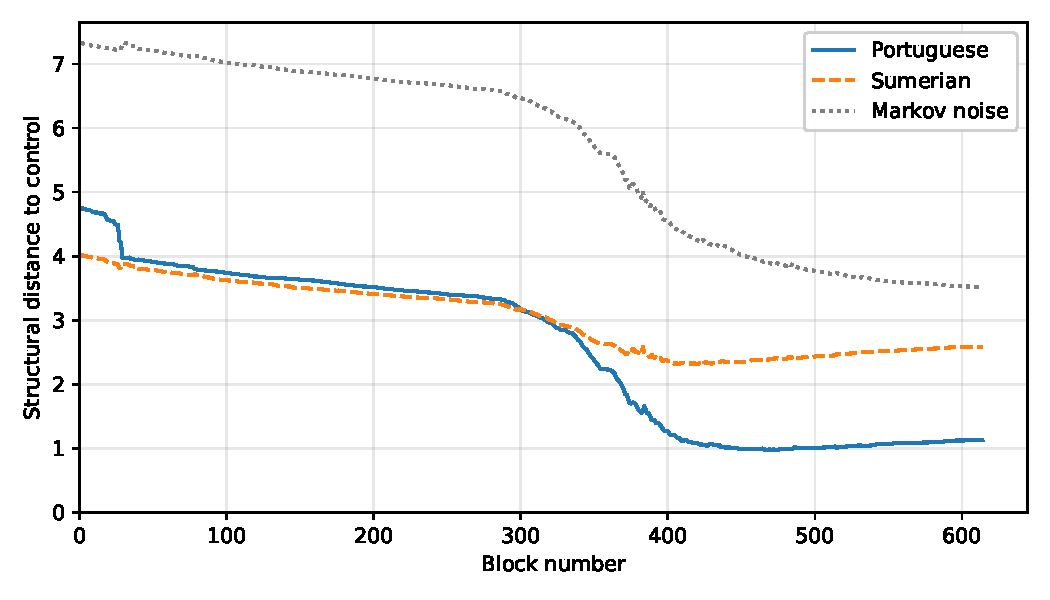
\includegraphics[width=\textwidth]{../../figures/Fig1}
\caption{Per-block structural distance from the synthetic corpus state to
each of the three controls (Portuguese, Sumerian, Markov noise) across the
614-block paper run. Portuguese reaches its minimum near block 470 at
$0.9730$. Sumerian reaches its minimum near block 408 at $2.3184$. Markov
noise reaches its minimum at the final block at $3.5248$. Portuguese is
never above the Sumerian curve in the second half of the run, but Sumerian
remains substantially closer to the synthetic state than Markov noise
throughout.}
\label{fig:controlbanktrajectory}
\end{figure}

\subsection{Dimensional robustness of the structural fingerprint}
\label{sec:dimensional-robustness}

The structural metric used in this paper operates in a four-dimensional
feature space. A natural question is whether the nearest-neighbor rankings
reported above are properties of the corpora or artifacts of compressing
inter-corpus structure into four dimensions. A post hoc dimensional
robustness check was performed against this concern; the full report is
stored at
\path{docs/reports/2026-05-19_dimensional_robustness_check.md} and the
numeric outputs at
\path{data/validation/2026-05-19_dimensional_robustness/}.

The check expanded the structural feature set to fifteen dimensions
(the original four plus eleven additional features: top-500 word bigram
and trigram coverage, top-1000 unigram coverage, sequence-length variance,
word-length mean and variance, hapax legomena ratio, Zipf slope over
ranks 10--1000, word bigram and trigram entropy, and suffix-profile
entropy), z-scored across the scored corpora, and recomputed cosine
distance to Latin under 4D, 10D, and 15D for the validator bank, the
control bank, and the v5 paper-run endpoint. The 4D scaled-Euclidean
distance from Modern Portuguese to block 0474 was reproduced exactly
($0.9729932421288967$), confirming that the expanded analysis uses the
same loading and feature path as the production scoring code.
Table~\ref{tab:dimrobust} reports the cosine distances under 4D and 15D,
sorted by 15D rank.

\begin{table}[h]
\centering
\caption{Cosine distance to Latin under 4D and 15D z-scored structural
feature spaces, sorted by 15D rank. The 4D space corresponds to the
production structural metric used in this paper; the 15D space adds
eleven Tier-1 and Tier-2 features documented in the robustness report.}
\label{tab:dimrobust}
\begin{tabular}{lrrrr}
\toprule
Corpus & 4D dist & 15D dist & 4D rank & 15D rank \\
\midrule
Modern Portuguese (withheld) & 0.813 & \textbf{0.334} & 7 & \textbf{1} \\
Modern French (source) & 0.812 & 0.577 & 6 & 2 \\
Old Occitan & 0.624 & 0.799 & 4 & 3 \\
Sumerian & 1.539 & 0.800 & 14 & 4 \\
Old French & 0.340 & 0.904 & 1 & 5 \\
Old Spanish & 1.001 & 0.954 & 10 & 6 \\
langue d'o\"il & 0.725 & 1.048 & 5 & 7 \\
Markov noise & 0.553 & 1.080 & 2 & 8 \\
Middle French & 1.062 & 1.091 & 11 & 9 \\
Anglo-Norman & 0.575 & 1.213 & 3 & 10 \\
\bottomrule
\end{tabular}
\end{table}

Principal-components analysis on the z-scored 15-feature matrix places
$95\%$ of inter-corpus variance in the first five components, with the
fifth component carrying $3.9\%$ and loading on top-1000 unigram coverage
and word-length mean, features that the original 4D space did not include.
The intrinsic dimensionality of inter-corpus structure for the corpora
scored here is therefore approximately five, not four.

\paragraph{The Sumerian result.}
The single most consequential observation from the dimensional expansion
is the position of Sumerian, a corpus originally selected as a control
because it was presumed unlikely to cluster near Latin under any meaningful
metric. This was not a result the run was designed to produce, and the
interpretation offered below is post hoc. In retrospect, it may not have
been the least rhetorically hazardous control language available; Japanese
or Quechua would have made the same typological point. Under 4D the metric placed it at rank 14,
last among the ten corpora; under 15D it rises to rank 4, inside the
medieval Romance cluster on structural proximity to Latin. Sumerian is
non-Indo-European, agglutinative, and historically unrelated to the
Romance line; no genealogical or contact-based account places Sumerian
closer to Latin than Old French or langue d'o\"il under any plausible
historical metric. Its rank-4 position under the richer feature space
is therefore consistent with reading the structural metric as a detector
of typological proximity (morphological richness, suffix-profile entropy,
inflectional vocabulary breadth) rather than genetic relationship or
historical contact. We treat this result as the strongest available
evidence against a purely genealogical reading of the metric. The
Portuguese-vs-medieval-validator comparison reported below is consistent
with that reading; the Sumerian rank is what rules out a purely
genealogical alternative.

The expansion produces two further consistent observations. First, the
Portuguese-vs-medieval-validator comparison strengthens rather than
weakens under expansion: the 4D space muted the Portuguese-Latin
proximity, and the eleven new features overwhelmingly pull Portuguese
further toward Latin. Second, the block-state ordering of v5 paper-run
checkpoints is preserved across all three dimensional settings: the
search did not climb an artifact of the 4D compression.

Reading the structural metric as a typological proximity detector rather
than a chronological one satisfies the three constraints articulated above.
The feature-space constraint is satisfied because typological proximity is
a plausible reading of what those four features collectively measure. The Portuguese constraint
is satisfied because Modern Portuguese has retained more Latin inflectional
morphology than Modern French has, and that retention manifests in TTR,
unigram coverage, word-length, and suffix-entropy axes. The path-bifurcation
constraint is satisfied because the structural and form axes measure
different properties (corpus-level morphological similarity versus
character-level surface similarity), which need not be co-monotonic on a
target-conditioned trajectory starting in a less-inflected modern descendant.
The interpretation is offered as the most parsimonious available reading
of the present data, not as a mechanistic claim about how Romance languages
stand to Latin.

\section{Limitations}

The present report is subject to the following constraints:

\begin{enumerate}
    \item The run is target-conditioned, not blind. Latin is in the active
    optimization loop.
    \item The validator bank currently contains six attested medieval Romance
    corpora. Token counts range from approximately 27{,}600 (Anglo-Norman) to
    80{,}000 (Old French).
    \item The Old Spanish validator corpus is dominated by a single author
    and genre: Gonzalo de Berceo's \emph{Milagros de Nuestra Se\~nora}
    (26 miracles plus prologue) plus the \emph{Poema de Mio Cid} fragment
    and related texts. The resulting fingerprint may reflect Berceo's
    individual style as much as the broader Old Spanish register.
    \item The control bank currently contains three controls only: Markov
    noise, Sumerian, and withheld Portuguese.
    \item The historical seed discrepancy has been resolved by replay audit,
    but the original launch path for the paper run did not preserve a
    self-consistent requested-seed versus engine-seed record at run time.
    \item The paper reports one source-target run only: French $\rightarrow$
    Latin.
    \item A three-seed early-window replication probe (seeds 42, 43, and 45,
    1{,}000 proposals each) found that all three seeds produced coherent,
    same-direction progress over the first block, with final structural scores
    in the range $-1.3614$ to $-1.3062$ and form scores in the range $0.6928$
    to $0.7181$. Seed~42 reproduced the historical paper-run block~0001 endpoint
    exactly. This probe supports the bounded claim that early-window behavior
    is not specific to a single seed; it does not establish whether the full
    long-horizon phase structure or the final plateau endpoint would replicate
    across seeds.
    \item The structural metric used during the paper run is four-dimensional.
    A post hoc dimensional robustness check
    (Section~\ref{sec:dimensional-robustness}) finds the intrinsic
    dimensionality of inter-corpus variance to be approximately five, so the
    4D space is slightly undersized for the full set of structural
    comparisons. The Portuguese-vs-medieval-validator comparison
    survives expansion to fifteen dimensions, but quantitative comparisons
    among the medieval validators themselves should be interpreted with
    caution, since some rank order changes under expansion.
    \item The family alignment score has a structural ceiling below $1.0$
    that depends on the target language. A post hoc self-similarity
    calibration finds the matched-slice ceiling for Latin to be $0.9583$:
    six of Latin's top-12 short-token families (\emph{in}, \emph{et},
    \emph{ut}, \emph{ad}, \emph{me}, \emph{si}) are 2-character tokens
    shorter than the suffix length used by the Hungarian alignment cost
    function, producing empty suffix profiles and a fixed self-cost of
    $0.0417$. The v5 endpoint family alignment score of $0.5139$ therefore
    represents approximately $54\%$ of the achievable Latin ceiling, not
    $51\%$ of nominal. Per-corpus ceilings vary between $0.9375$ and
    $0.9722$ depending on how many of each corpus's top-12 short-token
    families are 2-character entries; details are documented in
    \path{docs/reports/2026-05-19_latin_self_similarity_calibration.md}.
    \item Adversarial baselines beyond the Markov-noise null (feature
    ablations dropping individual structural components, shuffled
    feature-weight controls, synthetic-corpus controls preserving Zipf and
    length distributions, and randomized target-feature trajectories) were
    not run for this paper. The Markov, Sumerian, and Portuguese controls
    test that the optimizer finds non-trivial structure and that the
    structure is not lineage-tracking, but they do not test which individual
    features drive the structural metric. These ablations are a natural
    next experiment.
\end{enumerate}

\section{Conclusion}

The structural metric described in this paper appears to function as a
typological proximity detector rather than a chronological one. A post hoc
expansion of the structural feature space to fifteen dimensions
(Section~\ref{sec:dimensional-robustness}) preserved the
Portuguese-vs-medieval-validator comparison and additionally placed Sumerian,
a non-Indo-European agglutinative language with no historical relationship
to the Romance line, at fourth-rank structural proximity to Latin. The
instrument behavior reported here is consistent with that reading and does
not support mechanistic claims about Romance historical linguistics.

The run that produced this evidence was a complete French $\rightarrow$ Latin
retrodictive search under a frozen \emph{v5} configuration. The run halted by
plateau after 614{,}000 proposals and reached a near-zero Latin structural
score under the active metric. The best form checkpoint occurred earlier than
the final plateau endpoint. Post hoc validator-bank comparison reported a
structural nearest-neighbor path that oscillated between Middle French and
Old Spanish for the first 379 blocks before settling on Old Occitan through
the plateau endpoint, and a form nearest-neighbor path concentrated in Middle
French and other langue d'o\"il material, with the final block structurally
nearest to Old Occitan and form-wise nearest to Middle French.

Post hoc control-bank comparison reported a structural control path of
Sumerian $\rightarrow$ Portuguese and a form control path of Portuguese, while
Markov noise never became the nearest control on either axis. Withheld Modern
Portuguese reached a structural distance roughly twice as close to the final
block as the nearest medieval Romance validator, a gap that any
historical-reconstruction reading of the validator-bank chronology would need
to address.

\section*{Reproducibility Note}

The run manifest, preserved corpora, previews, block summaries, and
validator-bank outputs are stored in the repository. The paper-facing run
terminated by a native plateau rule rather than by manual truncation. A
post hoc replay audit resolved the historical seed mismatch for this run:
the manifest launch field records requested seed 45, while exact replay of
block 0001 identifies engine seed 42 as the seed actually used by the
search. The full audit is documented in
\path{docs/reports/2026-04-24_v5_paper_run_seed_audit.md}.
The validator-bank comparison files cited in this paper are stored under
\path{data/validation/french_v5_fortran_c16_seed45_paper_run_validator_bank_vs_validator_bank.*}.
The control-bank comparison files used for Figure~\ref{fig:controlbanktrajectory}
and Section~\ref{sec:dimensional-robustness} are stored under
\path{data/validation/french_v5_fortran_c16_seed45_paper_run_vs_control_bank.*}.
The post hoc dimensional robustness check is documented in
\path{docs/reports/2026-05-19_dimensional_robustness_check.md},
with numeric outputs under
\path{data/validation/2026-05-19_dimensional_robustness/}.
The Latin self-similarity calibration is documented in
\path{docs/reports/2026-05-19_latin_self_similarity_calibration.md},
with numeric outputs under
\path{data/validation/2026-05-19_self_similarity/}.

\section*{Competing Interests}

The author declares no competing interests.

\section*{Funding}

This work received no external funding.

\section*{Author Contributions}

T.O. designed the study, performed the analysis, and wrote the manuscript.

\section*{Use of AI Tools}

The author designed the methodology, experiments, and overall research
program. Claude Code (Anthropic) drafted most of the implementation,
including substantial portions of the engine
(\path{src/retrodiction/*.py}, \path{src/validation/*.py}), the
post hoc dimensional robustness check script
(\path{tmp_dimcheck/dim_robustness.py}), and the Latin
self-similarity calibration script
(\path{tmp_self_similarity/calibration.py}). Manuscript writing,
restructuring, and editing (including drafting of
Section~\ref{sec:dimensional-robustness}, the constraints paragraph in
\S3.5, the v5 objective equation in \S2.3, the Conclusion paragraph on
the typological-detector reading, the related-work expansion in \S1,
and the \S2.6 metric-scale clarification) were assisted by Claude
(Anthropic) operating in the Octave document-chat workstation. All AI
contributions followed prompts and specifications written by the author;
the author retains full responsibility for all design choices,
implementation correctness, analysis, and conclusions.

\bibliographystyle{plain}
\bibliography{references}

\end{document}
